% !TeX root = tcolorbox.tex
% include file of tcolorbox.tex (manual of the LaTeX package tcolorbox)
\clearpage
\section{Library 'skins'}\label{sec:skins}
The library is loaded by a package option or inside the preamble by:
\begin{dispListing}
\tcbuselibrary{skins}
\end{dispListing}
This also loads the package |tikz| \cite{tantau:2010c}. Typically but not necessarily,
the following skins use |tikz| instead of |pgf|.

\subsection{Technical Overview and Core Package Option Keys}\label{sec:skincorekeys}
From a technical point of view, a \emph{skin} is a style definition for the
appearance of a |tcolorbox|. The core package provides some additional
option keys for skins but only a single skin called \refSkin{standard}.
The 'skins' library adds several more skins. To change a skin, only one
option from the core package has to be set.

\begin{docTcbKey}{skin}{=\meta{name}}{style, no default, initially \texttt{standard}}
  Sets the current skin to \meta{name}. This is a style definition which sets all the following
  keys, i.\,e.\ for many use cases there is nothing more to do.
\begin{dispExample}
\tcbset{colback=Salmon!50!white,colframe=FireBrick!75!black,
  width=(\linewidth-8mm)/2,before=,after=\hfill,equal height group=ske}

\begin{tcolorbox}[adjusted title=My title]
  This is my content.
\end{tcolorbox}
\begin{tcolorbox}[skin=beamer,beamer,adjusted title=My title]
  This is my content.
\end{tcolorbox}
\end{dispExample}
\end{docTcbKey}


\begin{marker}
  On first read, you may skip the rest of this subsection and proceed to
  Subsection \ref{subsec:addstyleoptions} on page \pageref{subsec:addstyleoptions}.
  All following keys in this subsection are automatically set by the selected skin
  and you may never have to temper with them.
  Nevertheless, they can be used after a skin was selected to modify
  this skin.
\end{marker}


\begin{docTcbKey}{skin first}{=\meta{name}}{style, no default, initially \texttt{standard}}
  If the box is set to be \refKey{/tcb/breakable} and \emph{is} broken actually,
  then the skin for the \emph{first} part of the break sequence
  is set to \meta{name}, see Subsection \ref{subsec:breaksequence} on page \pageref{subsec:breaksequence}.
  Typically, this key is set by a \refKey{/tcb/skin}.
\end{docTcbKey}


\begin{docTcbKey}{skin middle}{=\meta{name}}{style, no default, initially \texttt{standard}}
  If the box is set to be \refKey{/tcb/breakable} and \emph{is} broken actually,
  then the skin for the \emph{middle} parts (if any) of the break sequence
  is set to \meta{name}, see Subsection \ref{subsec:breaksequence} on page \pageref{subsec:breaksequence}.
  Typically, this key is set by a \refKey{/tcb/skin}.
\end{docTcbKey}


\begin{docTcbKey}{skin last}{=\meta{name}}{style, no default, initially \texttt{standard}}
  If the box is set to be \refKey{/tcb/breakable} and \emph{is} broken actually,
  then the skin for the \emph{last} part of the break sequence
  is set to \meta{name}, see Subsection \ref{subsec:breaksequence} on page \pageref{subsec:breaksequence}.
  Typically, this key is set by a \refKey{/tcb/skin}.
\end{docTcbKey}




\begin{docTcbKey}{graphical environment}{=\meta{name}}{no default, initially \texttt{pgfpicture}}
  Sets the graphical environment for the |tcolorbox| to \meta{name}.
  Feasible values are |pgfpicture| and |tikzpicture| or environments which
  inherit from one of these two. This key is set by a \refKey{/tcb/skin} and
  may seldom be used directly.
\end{docTcbKey}

The skin of a |tcolorbox| is drawn by up to four \emph{engines}.
Afterwards, the text content is drawn which is not part of a skin.
The four steps are:
\begin{enumerate}
\item The \emph{frame} of the box.
\item The \emph{interior} of the box. The interior of a box with title is
  drawn differently from a box without title.
\item The \emph{segmentation} (line) of the box, if there is a lower part.
\item The \emph{title area} of the box, if there is a title.
\end{enumerate}

Every engine for the up to four steps can be set to one of the following types:
\begin{enumerate}
\item |standard|: the original code from the core package.
\item |path|: a |tikz| path which can be controlled by options.
\item |pathfirst|: a |tikz| path which can be controlled by options.
\item |pathmiddle|: a |tikz| path which can be controlled by options.
\item |pathlast|: a |tikz| path which can be controlled by options.
\item |freelance|: arbitrary user code.
\end{enumerate}
%\clearpage

\begin{docTcbKey}{frame engine}{=\meta{name}}{no default, initially \texttt{standard}}
  Sets the \emph{frame} drawing engine for a box to \meta{name}.
  Typically, this key is set by a \refKey{/tcb/skin}.
  Feasible values for \meta{name} are:
  \begin{itemize}
  \item |standard|: the original code from the core package,
  \item |path|: a |tikz| path which is controlled by \refKey{/tcb/frame style},
  \item |pathfirst|: a |tikz| path which is controlled by \refKey{/tcb/frame style},
  \item |pathmiddle|: a |tikz| path which is controlled by \refKey{/tcb/frame style},
  \item |pathlast|: a |tikz| path which is controlled by \refKey{/tcb/frame style},
  \item |freelance|: arbitrary user code which is given by \refKey{/tcb/frame code}.
  \end{itemize}
\end{docTcbKey}

\begin{docTcbKey}{interior titled engine}{=\meta{name}}{no default, initially \texttt{standard}}
  Sets the \emph{interior} drawing engine for a titled box to \meta{name}.
  Typically, this key is set by a \refKey{/tcb/skin}.
  Feasible values for \meta{name} are:
  \begin{itemize}
  \item |standard|: the original code from the core package,
  \item |path|: a |tikz| path which is controlled by \refKey{/tcb/interior style},
  \item |pathfirst|: a |tikz| path which is controlled by \refKey{/tcb/interior style},
  \item |pathmiddle|: a |tikz| path which is controlled by \refKey{/tcb/interior style},
  \item |pathlast|: a |tikz| path which is controlled by \refKey{/tcb/interior style},
  \item |freelance|: arbitrary user code which is given by \refKey{/tcb/interior titled code}.
  \end{itemize}
\end{docTcbKey}

\begin{docTcbKey}{interior engine}{=\meta{name}}{no default, initially \texttt{standard}}
  Sets the \emph{interior} drawing engine for an untitled box to \meta{name}.
  Typically, this key is set by a \refKey{/tcb/skin}.
  Feasible values for \meta{name} are:
  \begin{itemize}
  \item |standard|: the original code from the core package,
  \item |path|: a |tikz| path which is controlled by \refKey{/tcb/interior style},
  \item |pathfirst|: a |tikz| path which is controlled by \refKey{/tcb/interior style},
  \item |pathmiddle|: a |tikz| path which is controlled by \refKey{/tcb/interior style},
  \item |pathlast|: a |tikz| path which is controlled by \refKey{/tcb/interior style},
  \item |freelance|: arbitrary user code which is given by \refKey{/tcb/interior code}.
  \end{itemize}
\end{docTcbKey}

\begin{docTcbKey}{segmentation engine}{=\meta{name}}{no default, initially \texttt{standard}}
  Sets the \emph{segmentation} (line) drawing engine for a box to \meta{name}.
  Typically, this key is set by a \refKey{/tcb/skin}.
  Feasible values for \meta{name} are:
  \begin{itemize}
  \item |standard|: the original code from the core package,
  \item |path|: a |tikz| path which is controlled by \refKey{/tcb/segmentation style},
  \item |freelance|: arbitrary user code which is given by \refKey{/tcb/segmentation code}.
  \end{itemize}
\end{docTcbKey}

\begin{docTcbKey}{title engine}{=\meta{name}}{no default, initially \texttt{standard}}
  Sets the \emph{title area} drawing engine for a titled box to \meta{name}.
  Typically, this key is set by a \refKey{/tcb/skin}.
  Feasible values for \meta{name} are:
  \begin{itemize}
  \item |standard|: the original code from the core package,
  \item |path|: a |tikz| path which is controlled by \refKey{/tcb/title style},
  \item |pathfirst|: a |tikz| path which is controlled by \refKey{/tcb/title style},
  \item |pathmiddle|: a |tikz| path which is controlled by \refKey{/tcb/title style},
  \item |pathlast|: a |tikz| path which is controlled by \refKey{/tcb/title style},
  \item |freelance|: arbitrary user code which is given by \refKey{/tcb/title code}.
  \end{itemize}
\end{docTcbKey}

\begin{docTcbKey}{geometry nodes}{\colOpt{=\meta{boolean value}}}{default |true|, initially |false|}
  If set to |true|, up to four |tikz| nodes are defined for a |tcolorbox|
  which are named |frame|, |interior|, |segmentation|, and |title|. These nodes
  describe the boundaries of the equally named parts of a |tcolorbox|.
  They are used by all engines of type |path| and they may be used by engines
  of type |freelance|. Typically, this key is set by a \refKey{/tcb/skin}.
\begin{dispExample}
\tcbset{colback=Salmon!50!white,colframe=FireBrick!75!black,
  width=(\linewidth-8mm)/2,before=,after=\hfill,equal height group=geon}

\begin{tcolorbox}[adjusted title=The title]
  The upper part.\tcblower The lower part.
\end{tcolorbox}
\begin{tcolorbox}[adjusted title=The title,skin=freelance,
  frame code={\path[draw=red,fill=red!25]
      (frame.south west) rectangle (frame.north east);},
  interior titled code={\path[draw=blue,fill=blue!25]
      (interior.south west) rectangle (interior.north east);},
  segmentation code={\path[draw=green,fill=green!25]
      (segmentation.south west) rectangle (segmentation.north east);},
  title code={\path[draw=black,fill=brown!75!black]
      (title.south west) rectangle (title.north east);}]
  The upper part.\tcblower The lower part.
\end{tcolorbox}
\end{dispExample}
\end{docTcbKey}


\clearpage
\subsection{Style Option Keys}\label{subsec:addstyleoptions}
The following style options are applicable for all skins which
use engines of type |path|, |pathfirst|, |pathmiddle|, or |pathlast|.
Especially, the skin \refSkin{enhanced} supports \emph{all} of them
and \refSkin{standard} \emph{none}.

\begin{docTcbKey}{frame style}{=\meta{\texttt{\upshape tikz} keys}}{style, no default}
  The \meta{\texttt{\upshape tikz} keys} are used inside the |tikz| path command
  for drawing the \emph{frame} of the box.\\
  This option is available if the \refKey{/tcb/frame engine} is set to
  |path|, |pathfirst|, |pathmiddle|, or |pathlast|.
  It is \emph{not} available for |standard| and it \emph{may} be
  applicable for |freelance|.
\begin{dispExample*}{sbs,lefthand ratio=0.66}
\tcbset{colback=red!5!white,fonttitle=\bfseries}

\begin{tcolorbox}[enhanced,title=My title,
  frame style={left color=red!75!black,
               right color=blue!75!black}]
This is a \textbf{tcolorbox}.
\tcblower
This is the lower part.
\end{tcolorbox}
\end{dispExample*}
\end{docTcbKey}


\begin{docTcbKey}{frame hidden}{}{style, no value}
  This is a shortcut for |frame style={draw=none,fill=none}|.
  Depending on the skin, this option switches off the drawing of the
  frame.
\begin{dispExample*}{sbs,lefthand ratio=0.66}
\tcbset{colback=red!5!white,colframe=red!75!black,
  fonttitle=\bfseries,coltitle=black}

\begin{tcolorbox}[enhanced,title=My title,
  frame hidden]
This is a \textbf{tcolorbox}.
\tcblower
This is the lower part.
\end{tcolorbox}
\end{dispExample*}
\end{docTcbKey}


\begin{docTcbKey}{interior style}{=\meta{\texttt{\upshape tikz} keys}}{style, no default}
  The \meta{\texttt{\upshape tikz} keys} are used inside the |tikz| path command
  for drawing the \emph{interior} of the box. They are used for the titled
  and for the untitled version as well.\\
  This option is available if the \refKey{/tcb/interior titled engine}
  or \refKey{/tcb/interior engine} is set to
  |path|, |pathfirst|, |pathmiddle|, or |pathlast|.
  It is \emph{not} available for |standard| and it \emph{may} be
  applicable for |freelance|.
\begin{dispExample*}{sbs,lefthand ratio=0.66}
\tcbset{colframe=red!75!black,fonttitle=\bfseries}

\begin{tcolorbox}[enhanced,title=My title,
  interior style={left color=red!20!white,
                  right color=yellow!50!white}]
This is a \textbf{tcolorbox}.
\tcblower
This is the lower part.
\end{tcolorbox}
\end{dispExample*}
\end{docTcbKey}

\clearpage

\begin{docTcbKey}{interior hidden}{}{style, no value}
  This is a shortcut for |interior style={draw=none,fill=none}|.
  Depending on the skin, this option switches off the drawing of the
  interior.
\begin{dispExample*}{sbs,lefthand ratio=0.66}
\tcbset{frame style={top color=red!20!white,
  bottom color=red!20!white!75!black},
  fonttitle=\bfseries,coltitle=black}

\begin{tcolorbox}[enhanced,title=My title,
  interior hidden]
This is a \textbf{tcolorbox}.
\tcblower
This is the lower part.
\end{tcolorbox}
\end{dispExample*}
\end{docTcbKey}


\begin{docTcbKey}{segmentation style}{=\meta{\texttt{\upshape tikz} keys}}{style, no default}
  The \meta{\texttt{\upshape tikz} keys} are used inside the |tikz| path command
  for drawing the \emph{segmentation} line of the box.\\
  This option is available if the \refKey{/tcb/segmentation engine}
  is set to |path|.
  It is \emph{not} available for |standard| and it \emph{may} be
  applicable for |freelance|.
\begin{dispExample*}{sbs,lefthand ratio=0.66}
\tcbset{colback=red!5!white,colframe=red!75!black,
  fonttitle=\bfseries}

\begin{tcolorbox}[enhanced,title=My title,
  segmentation style={double=white,draw=blue,
                  double distance=1pt,solid}]
This is a \textbf{tcolorbox}.
\tcblower
This is the lower part.
\end{tcolorbox}
\end{dispExample*}
\end{docTcbKey}


\begin{docTcbKey}{segmentation hidden}{}{style, no value}
  This is a shortcut for |segmentation style={draw=none,fill=none}|.
  Depending on the skin, this option switches off the drawing of the
  segmentation line. See also \refKey{/tcb/lower separated} which
  has the same effect for most skins.
\begin{dispExample*}{sbs,lefthand ratio=0.66}
\tcbset{colback=red!5!white,colframe=red!75!black,
  fonttitle=\bfseries}

\begin{tcolorbox}[title=My title,
  enhanced,segmentation hidden]
This is a \textbf{tcolorbox}.
\tcblower
This is the lower part.
\end{tcolorbox}
\end{dispExample*}
\end{docTcbKey}


\clearpage
\begin{docTcbKey}{title style}{=\meta{\texttt{\upshape tikz} keys}}{style, no default}
  The \meta{\texttt{\upshape tikz} keys} are used inside the |tikz| path command
  for drawing the \emph{title area} of the box.\\
  This option is available if the \refKey{/tcb/title engine} is set to
  |path|, |pathfirst|, |pathmiddle|, or |pathlast|.
  It is \emph{not} available for |standard| and it \emph{may} be
  applicable for |freelance|.
\begin{dispExample*}{sbs,lefthand ratio=0.66}
\tcbset{colback=red!5!white,colframe=red!75!black,
  coltitle=blue!50!black,fonttitle=\bfseries}

\begin{tcolorbox}[enhanced,title=My title,
  title style={left color=blue!15!yellow,
               right color=red!85!black}]
This is a \textbf{tcolorbox}.
\tcblower
This is the lower part.
\end{tcolorbox}
\end{dispExample*}
\end{docTcbKey}


\begin{docTcbKey}{colbacktitle}{=\meta{color}}{style, no default, initially unset}
  Abbreviation for setting \refKey{/tcb/title style} to |fill=|\meta{color}.
  This fills the background of the title area with the given \meta{color}.\\
  This option is available if the \refKey{/tcb/title engine} is set to
  |path|, |pathfirst|, |pathmiddle|, or |pathlast|.
  It is \emph{not} available for |standard| and it \emph{may} be
  applicable for |freelance|.
\begin{dispExample*}{sbs,lefthand ratio=0.66}
\tcbset{colback=red!5!white,colframe=red!75!black,
  coltitle=blue!50!black,fonttitle=\bfseries}

\begin{tcolorbox}[enhanced,title=My title,
  colbacktitle=yellow!50!white]
This is a \textbf{tcolorbox}.
\tcblower
This is the lower part.
\end{tcolorbox}
\end{dispExample*}
\end{docTcbKey}


\begin{docTcbKey}{title hidden}{}{style, no value}
  This is a shortcut for |title style={draw=none,fill=none}|.
  Depending on the skin, this option switches off the drawing of the
  title background. This is the default behavior for \refSkin{standard} and
  \refSkin{enhanced}.
\begin{dispExample*}{sbs,lefthand ratio=0.66}
\tcbset{colback=red!5!white,colframe=red!75!black,
  fonttitle=\bfseries}

\begin{tcolorbox}[title=My title,
  enhanced,title hidden]
This is a \textbf{tcolorbox}.
\tcblower
This is the lower part.
\end{tcolorbox}
\end{dispExample*}
\end{docTcbKey}


\clearpage
\subsection{Code Option Keys}\label{subsec:addcodeoptions}
The following code options are applicable for all skins which
use engines of type |freelance|.
Especially, the skin \refSkin{freelance} supports \emph{all} of them,
\refSkin{standard} and \refSkin{enhanced} \emph{none} of them.


\begin{docTcbKey}{frame code}{\colOpt{=\meta{graphical code}}}{code, default from |standard|}
  The given \meta{graphical code} is used for drawing the \emph{frame} of the box.\\
  This option is available only if the \refKey{/tcb/frame engine} is set to |freelance|.
\begin{dispExample}
\tcbset{colback=red!5!white,colframe=red!75!black}

\begin{tcolorbox}[freelance,frame code={
  \foreach \n in {north east,north west,south east,south west}
  {\path [fill=red!75!black] (interior.\n) circle (3mm); }; }]
This is a \textbf{tcolorbox}.
\tcblower
This is the lower part.
\end{tcolorbox}
\end{dispExample}
\end{docTcbKey}

\begin{docTcbKey}{interior titled code}{\colOpt{=\meta{graphical code}}}{code, default from |standard|}
  The given \meta{graphical code} is used
  for drawing the \emph{interior} of the box, if the box comes with a title.\\
  This option is available only if the \refKey{/tcb/interior titled engine} is set to |freelance|.
\begin{dispExample}
\tcbset{colback=red!5!white,colframe=red!75!black,fonttitle=\bfseries}

\begin{tcolorbox}[freelance,title=My title,interior titled code={
  \path[draw=red!5!white,line width=5mm,line cap=round]
    ([xshift=3mm,yshift=-3mm]interior.north west)
    --([xshift=-3mm,yshift=3mm]interior.south east)
    ([xshift=3mm,yshift=3mm]interior.south west)
    --([xshift=-3mm,yshift=-3mm]interior.north east);}]
This is a \textbf{tcolorbox}.
\tcblower
This is the lower part.
\end{tcolorbox}
\end{dispExample}
\end{docTcbKey}


\clearpage
\begin{docTcbKey}{interior code}{\colOpt{=\meta{graphical code}}}{code, default from |standard|}
  The given \meta{graphical code} is used
  for drawing the \emph{interior} of the box, if the box is without a title.\\
  This option is available only if the \refKey{/tcb/interior engine} is set to |freelance|.
\begin{dispExample}
\tcbset{colback=red!5!white,colframe=red!75!black}

\begin{tcolorbox}[freelance,interior code={
  \path[draw=red!5!white,line width=5mm,line cap=round]
    ([xshift=3mm,yshift=-3mm]interior.north west)
    --([xshift=-3mm,yshift=3mm]interior.south east)
    ([xshift=3mm,yshift=3mm]interior.south west)
    --([xshift=-3mm,yshift=-3mm]interior.north east);}]
This is a \textbf{tcolorbox}.
\tcblower
This is the lower part.
\end{tcolorbox}
\end{dispExample}
\end{docTcbKey}

\begin{docTcbKey}{segmentation code}{\colOpt{=\meta{graphical code}}}{code, default from |standard|}
  The given \meta{graphical code} is used for drawing the
  \emph{segmentation} area of the box.\\
  This option is available only if the \refKey{/tcb/segmentation engine} is set to |freelance|.
\begin{dispExample}
\tcbset{colback=red!5!white,colframe=red!75!black,fonttitle=\bfseries}

\begin{tcolorbox}[freelance,title=My title,segmentation code={
  \path[top color=red!5!white,bottom color=red!5!white,middle color=blue]
  (segmentation.south west) rectangle (segmentation.north east);}]
This is a \textbf{tcolorbox}.
\tcblower
This is the lower part.
\end{tcolorbox}
\end{dispExample}
\end{docTcbKey}


\clearpage
\begin{docTcbKey}{title code}{\colOpt{=\meta{graphical code}}}{code, default from |standard|}
  The given \meta{graphical code} is used for drawing the
  \emph{title} area of the box.\\
  This option is available only if the \refKey{/tcb/title engine} is set to |freelance|.
\begin{dispExample}
\tcbset{colback=red!5!white,colframe=red!75!black,fonttitle=\bfseries,
  coltitle=black}

\begin{tcolorbox}[freelance,title=My title,title code={
  \path[draw=yellow,solid,decorate,line width=2mm,
    decoration={coil,aspect=0,segment length=10.1mm}]
    ([xshift=1mm]title.west) -- ([xshift=-1mm]title.east);}]
This is a \textbf{tcolorbox}.
\tcblower
This is the lower part.
\end{tcolorbox}
\end{dispExample}
\end{docTcbKey}


\clearpage
\subsection{Watermark Option Keys}\label{subsec:watermarks}
The following watermark options are applicable for all skins which
use |tikzpicture| as \refKey{/tcb/graphical environment}.
Therefore, the skin \refSkin{standard} does not support these watermarks,
but all other skins, e.\,g.\ \refSkin{enhanced}.

\begin{marker}
The watermark options rely on the more general overlay options described in
Section \ref{subsec:overlays} from page \pageref{subsec:overlays}.
Therefore, \emph{watermarks} and \emph{overlays} cannot be used mixed.
But a mixture is possible with the 'hooks' library, see Section \ref{sec:hooks}.
\end{marker}


\begin{docTcbKey}{watermark text}{=\meta{text}}{no default, initially unset}
  Writes some \meta{text} in the center of the interior region of a |tcolorbox|.
  This \meta{text} is written \emph{after} the
  frame and interior are drawn and \emph{before} the text content is drawn.
  It is zoomed or stretched according the values of
  \refKey{/tcb/watermark zoom} or \refKey{/tcb/watermark stretch}.
\begin{dispExample}
\tcbset{colback=red!5!white,colframe=red!75!black,fonttitle=\bfseries}

\begin{tcolorbox}[enhanced,title=My title,watermark text=My Watermark]
\lipsum[1]
\tcblower
\lipsum[2]
\end{tcolorbox}
\end{dispExample}
\end{docTcbKey}


\begin{docTcbKey}{watermark text on}{=\meta{part} is \meta{text}}{no default, initially unset}
  This option writes some \meta{text} in the center of the interior region of a |tcolorbox|
  as described for \refKey{/tcb/watermark text}.
  But this is done only for boxes named \meta{part} of a break sequence, see
  \refKey{/tcb/breakable}.\\ 
  Feasible values for \meta{part} are:
  \begin{itemize}
  \item |broken|: all broken box parts,
  \item |unbroken|: unbroken boxes only,
  \item |first|: first parts of a break sequence,
  \item |middle|: middle parts of a break sequence,
  \item |last|: last parts of a break sequence,
  \item |unbroken and first|: unbroken boxes and first parts of a break sequence,
  \item |middle and last|: middle and last parts of a break sequence.
  \end{itemize}
\end{docTcbKey}


\clearpage


\begin{docTcbKey}{watermark graphics}{=\meta{file name}}{no default, initially unset}
  Draws an external picture referenced by \meta{file name}
  in the center of the interior region of a |tcolorbox|.
  The picture is drawn \emph{after} the
  frame and interior are drawn and \emph{before} the text content is drawn.
  It is zoomed or stretched according the values of
  \refKey{/tcb/watermark zoom} or \refKey{/tcb/watermark stretch}.
\begin{dispExample}
\tcbset{colback=red!5!white,colframe=red!75!black,fonttitle=\bfseries}

\begin{tcolorbox}[enhanced,title=My title,watermark graphics=Basilica_5.png,
  watermark opacity=0.15]
\lipsum[1-2]
\tcblower
This example uses a public domain picture from\\
\url{http://commons.wikimedia.org/wiki/File:Basilica_5.png}
\end{tcolorbox}
\end{dispExample}
\end{docTcbKey}


\begin{docTcbKey}{watermark graphics on}{=\meta{part} is \meta{file name}}{no default, initially unset}
  This option draws a picture referenced by \meta{file name} in the center of the interior region of a |tcolorbox|
  as described for \refKey{/tcb/watermark graphics}.
  But this is done only for boxes named \meta{part} of a break sequence, see
  \refKey{/tcb/breakable}.\\ 
  Feasible values for \meta{part} are:
  \begin{itemize}
  \item |broken|: all broken box parts,
  \item |unbroken|: unbroken boxes only,
  \item |first|: first parts of a break sequence,
  \item |middle|: middle parts of a break sequence,
  \item |last|: last parts of a break sequence,
  \item |unbroken and first|: unbroken boxes and first parts of a break sequence,
  \item |middle and last|: middle and last parts of a break sequence.
  \end{itemize}
\end{docTcbKey}



\clearpage
\begin{docTcbKey}{watermark tikz}{=\meta{graphical code}}{no default, initially unset}
  Draws the given |tikz| \meta{graphical code}
  in the center of the interior region of a |tcolorbox|.
  The code is executed \emph{after} the
  frame and interior are drawn and \emph{before} the text content is drawn.
  The result is zoomed or stretched according the values of
  \refKey{/tcb/watermark zoom} or \refKey{/tcb/watermark stretch}.
\begin{dispExample}
\tcbset{colback=red!5!white,colframe=red!75!black,fonttitle=\bfseries}

\begin{tcolorbox}[enhanced,title=My title,
  watermark tikz={\draw[line width=2mm] circle (1cm)
    node{\fontfamily{ptm}\fontseries{b}\fontsize{20mm}{20mm}\selectfont ?};}]
\lipsum[1]
\tcblower
\lipsum[2]
\end{tcolorbox}
\end{dispExample}
\end{docTcbKey}



\begin{docTcbKey}{watermark tikz on}{=\meta{part} is \meta{graphical code}}{no default, initially unset}
  This option draws the given |tikz| \meta{graphical code} in the center of the interior region of a |tcolorbox|
  as described for \refKey{/tcb/watermark tikz}.
  But this is done only for boxes named \meta{part} of a break sequence, see
  \refKey{/tcb/breakable}.\\ 
  Feasible values for \meta{part} are:
  \begin{itemize}
  \item |broken|: all broken box parts,
  \item |unbroken|: unbroken boxes only,
  \item |first|: first parts of a break sequence,
  \item |middle|: middle parts of a break sequence,
  \item |last|: last parts of a break sequence,
  \item |unbroken and first|: unbroken boxes and first parts of a break sequence,
  \item |middle and last|: middle and last parts of a break sequence.
  \end{itemize}
\end{docTcbKey}


\begin{docTcbKey}{no watermark}{}{style, no default, initially set}
  Removes the watermark if set before. This is an alias for
  \refKey{/tcb/no overlay}.
\end{docTcbKey}


\clearpage
\begin{docTcbKey}{watermark opacity}{=\meta{fraction}}{no default, initially |1.00|}
  Sets the opacity value $\in[0,1]$ for a watermark.
\begin{dispExample}
\tcbset{enhanced,colback=red!5!white,colframe=red!75!black,fonttitle=\bfseries,
  watermark text=Watermark,nobeforeafter,width=(\linewidth-2mm)/2}

\begin{tcolorbox}[title=Opacity 1.00,watermark opacity=1.00]
\lipsum[2]
\end{tcolorbox}\hfill%
\begin{tcolorbox}[title=Opacity 0.50,watermark opacity=0.50]
\lipsum[2]
\end{tcolorbox}%
\end{dispExample}
\end{docTcbKey}

\enlargethispage{5mm}
\begin{docTcbKey}{watermark zoom}{=\meta{fraction}}{no default, initially |0.75|}
  Sets the zoom value for a watermark. The zoom respects the aspect ratio.
  The value $1.0$ means to fill the whole box until the watermark touches the frame.
\begin{dispExample}
\tcbset{enhanced,colback=red!5!white,colframe=red!75!black,fonttitle=\bfseries,
  watermark text=Watermark,nobeforeafter,width=(\linewidth-2mm)/2}

\begin{tcolorbox}[title=Zoom 1.0,watermark zoom=1.0]
\lipsum[2]
\end{tcolorbox}\hfill%
\begin{tcolorbox}[title=Zoom 0.5,watermark zoom=0.5]
\lipsum[2]
\end{tcolorbox}%
\end{dispExample}
\end{docTcbKey}

\clearpage

\begin{docTcbKey}{watermark overzoom}{=\meta{fraction}}{no default, initially unset}
  Sets the overzoom value for a watermark. The overzoom respects the aspect ratio.
  The value $1.0$ means to fill the whole box until the watermark touches
  all four sides of the frame.
\begin{dispExample}
\tcbset{enhanced,colback=white,colframe=blue!50!black,fonttitle=\bfseries,
  watermark opacity=0.5,
  watermark graphics=lichtspiel.jpg,nobeforeafter,width=(\linewidth-2mm)/2}

\begin{tcolorbox}[title=Zoom 1.0,watermark zoom=1.0]
\lipsum[1]
\end{tcolorbox}\hfill%
\begin{tcolorbox}[title=Overzoom 1.0,watermark overzoom=1.0]
\lipsum[1]
\end{tcolorbox}%
\end{dispExample}
\end{docTcbKey}

\begin{marker}
If a \refKey{/tcb/watermark overzoom} value of |1.0| is used in connection
with invisible top and bottom rules which still have a thickness greater than |0pt|,
the space of these invisible rules may not be covered by the watermark.
For example, this situation may occur during the breaking of \refKey{/tcb/enhanced} boxes.
To avoid this optical glitch, just set \refKey{/tcb/pad at break} to any desired value.
\end{marker}

\clearpage
\begin{docTcbKey}{watermark stretch}{=\meta{fraction}}{no default, initially unset}
  Sets the stretch value for a watermark. The stretch value is applied to width
  and height in relation to the box dimensions. It does not respect the aspect ratio.
  The value $1.0$ means to fill the whole box.
\begin{dispExample}
\tcbset{enhanced,colback=white,colframe=blue!50!black,fonttitle=\bfseries,
  watermark graphics=lichtspiel.jpg,watermark opacity=0.5,
  nobeforeafter,width=(\linewidth-2mm)/2}

\begin{tcolorbox}[title=Stretch 1.00,watermark stretch=1.00]
\lipsum[2]
\end{tcolorbox}\hfill%
\begin{tcolorbox}[title=Stretch 0.50,watermark stretch=0.50]
\lipsum[2]
\end{tcolorbox}%
\end{dispExample}
\end{docTcbKey}

\begin{docTcbKey}{watermark color}{=\meta{color}}{no default, initially mixed background and frame color}
  Sets the color for the watermark.
\begin{dispExample}
\tcbset{colback=red!5!white,colframe=red!75!black,fonttitle=\bfseries}

\begin{tcolorbox}[enhanced,title=My title,watermark text=My Watermark,
  watermark color=yellow!50!red]
\lipsum[1]
\end{tcolorbox}
\end{dispExample}
\end{docTcbKey}

\clearpage

\begin{docTcbKey}{clip watermark}{\colOpt{=\meta{boolean value}}}{default |true|, initially |true|}
  Sets the watermark to be clipped to the interior area.
\begin{dispExample}
\tcbset{enhanced,colback=white,colframe=blue!50!white,fonttitle=\bfseries,
  watermark opacity=0.5,watermark stretch=1.00,arc=3mm,
  watermark graphics=lichtspiel.jpg}

\begin{tcolorbox}[title=Clip (default),clip watermark]
\lipsum[1]
\end{tcolorbox}

\begin{tcolorbox}[title=No clip,clip watermark=false]
\lipsum[1]
\end{tcolorbox}%
\end{dispExample}
\end{docTcbKey}



\clearpage
\subsection{Clip Environments}\label{subsec:clipping}
The following clip environments are applicable for all skins which
use engines of type |path|, |pathfirst|, |pathmiddle|, or |pathlast|.
Especially, the skin \refSkin{enhanced} supports \emph{all} of them
and \refSkin{standard} \emph{none}. The typical area of application
is inside overlay code, see Section \ref{subsec:overlays} from
page \pageref{subsec:overlays}.


\begin{docEnvironment}{tcbclipframe}{}
Defines a |Tikz| scope which clips to the frame area path.
\begin{dispExample}
\makeatletter
\newtcolorbox{picturebox}[2][]{%
  enhanced,frame hidden,interior hidden,fonttitle=\bfseries,
  overlay={\begin{tcbclipframe}\node at (frame)
    {\includegraphics[width=\tcb@width,height=\tcb@height]{#2}};\end{tcbclipframe}%
    \begin{tcbclipinterior}\fill[white,opacity=0.75]
    (frame.south west) rectangle (frame.north east);\end{tcbclipinterior}},#1}
\makeatother

\begin{picturebox}[title=My Picture Box]{lichtspiel.jpg}
\lipsum[1]
\end{picturebox}
\end{dispExample}
\end{docEnvironment}

\clearpage
\begin{docEnvironment}{tcbclipinterior}{}
Defines a |Tikz| scope which clips to the interior area path.
\begin{dispExample}
\begin{tcolorbox}[enhanced,title=My Title,
  overlay={\begin{tcbclipinterior}
    \draw[red,line width=1cm] (interior.north west)--(interior.south east);
    \draw[red,line width=1cm] (interior.south west)--(interior.north east);
  \end{tcbclipinterior}}]
\lipsum[1]
\end{tcolorbox}
\end{dispExample}
\end{docEnvironment}

\begin{docEnvironment}{tcbcliptitle}{}
Defines a |Tikz| scope which clips to the title area path.
\begin{dispExample}
\begin{tcolorbox}[enhanced,title=My Title,colframe=blue,colback=yellow!10!white,
  overlay={\begin{tcbcliptitle}\node at (title)
  {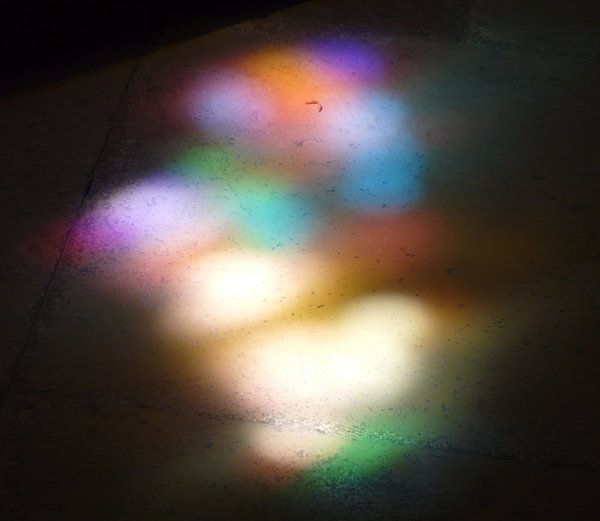
\includegraphics[width=\linewidth]{lichtspiel.jpg}};\end{tcbcliptitle}}]
\lipsum[1]
\end{tcolorbox}
\end{dispExample}
\end{docEnvironment}

\clearpage
\begin{docTcbKey}{clip title}{\colOpt{=\meta{boolean value}}}{default |true|, initially |false|}
  Sets the title to be clipped to the title area.
\begin{dispExample}
\tcbset{enhanced,width=5cm,colframe=red!50!white,coltitle=black}

\begin{tcolorbox}[title=\mbox{This is a title which is unbreakable and far too long}]
This is a tcolorbox.
\end{tcolorbox}

\begin{tcolorbox}[title=\mbox{This is a title which is unbreakable and far too long},
  clip title]
This is a tcolorbox.
\end{tcolorbox}
\end{dispExample}
\end{docTcbKey}


\begin{docTcbKey}{clip upper}{\colOpt{=\meta{boolean value}}}{default |true|, initially |false|}
  Sets the upper part to be clipped to the interior area.
\begin{dispExample}
\newcommand{\mygraphics}[2][]{%
  \tcbox[enhanced,boxsep=0pt,top=0pt,bottom=0pt,left=0pt,
    right=0pt,boxrule=0.4pt,drop fuzzy shadow,clip upper,
    colback=black!75!white,toptitle=2pt,bottomtitle=2pt,nobeforeafter,
    center title,fonttitle=\small\sffamily,title=\detokenize{#2}]
  {\includegraphics[width=\the\dimexpr(\linewidth-4mm)/2\relax]{#2}}}

\mygraphics{lichtspiel.jpg}\hfill
\mygraphics{Basilica_5.png}
\end{dispExample}
\end{docTcbKey}

\clearpage
The example for \refKey{/tcb/clip upper} sizes the box according to
the dimensions of the picture. To do it the other way around, the watermark
options provide an easy solution.
\begin{dispExample}
\newcommand{\mygraphics}[2][]{%
  \tcbox[enhanced,capture=minipage,boxsep=0pt,top=0pt,bottom=0pt,left=0pt,
    right=0pt,boxrule=0.4pt,drop fuzzy shadow,nobeforeafter,
    colback=black!75!white,toptitle=2pt,bottomtitle=2pt,
    center title,fonttitle=\small\sffamily,title=\detokenize{#2},
    width=(\linewidth-4mm)/2,height=6cm,colbacktitle={black},
    watermark zoom=1.0,watermark graphics={#2}]{}}

\mygraphics{lichtspiel.jpg}\hfill
\mygraphics{Basilica_5.png}
\end{dispExample}


\begin{docTcbKey}{clip lower}{\colOpt{=\meta{boolean value}}}{default |true|, initially |false|}
  Sets the lower part to be clipped to the interior area.
\begin{dispExample}
\tcbset{enhanced,width=5cm,colframe=red!50!black,text and listing}

\begin{tcblisting}{}
Donau\-dampf\-schiff\-fahrts\-ka\-pi\-t\"ans\-m\"ut\-zen\-fran\-sen
\end{tcblisting}

\begin{tcblisting}{clip lower}
Donau\-dampf\-schiff\-fahrts\-ka\-pi\-t\"ans\-m\"ut\-zen\-fran\-sen
\end{tcblisting}
\end{dispExample}
\end{docTcbKey}


\clearpage
\subsection{Border Line Option Keys}\label{subsec:borderline}
The following border line options are applicable for most skins which
use |tikzpicture| as \refKey{/tcb/graphical environment}.
Therefore, the skin \refSkin{standard} does not support these border lines,
but most other skins, e.\,g.\ \refSkin{enhanced}.

The border lines are independent from the normal |tcolorbox| rules.
They may be used with or without the \refKey{/tcb/segmentation engine}.

The border lines are stackable, i.\,e.\ several different border lines can be
used on the same |tcolorbox|. They are drawn \emph{after} the box frame and box
interior and \emph{before} overlays or watermarks.

\begin{marker}
Technically, the normal |tcolorbox| rules result from a TikZ \emph{filling}
process. The border lines are created by a TikZ \emph{drawing} process.
This can be used to apply different effects.
\end{marker}


\begin{docTcbKey}{borderline}{=\marg{width}\marg{offset}\marg{options}}{no default, initially unset}
  Adds a new border line to the stack of border lines.
  This border line is drawn with the given \meta{width} and gets a
  \meta{offset} computed from the frame outline. A positive \meta{offset} value
  moves the borderline inside the |tcolorbox| and a negative \meta{offset} value
  moves it outside without changing the bounding box.\\
  The border line is drawn along a TikZ path with the given TikZ \meta{options}.
  Note that the TikZ |line width| option should not be used here.\\
  The border lines adapt to the rounded corners of the |tcolorbox|. An inside border
  line will switch to sharp corners if necessary, an outside border line will
  always be rounded if not set to |sharp corners|.
\begin{dispExample}
\begin{tcolorbox}[enhanced,title=Rounded corners,fonttitle=\bfseries,boxsep=5pt,
  arc=8pt,
  borderline={0.5pt}{0pt}{red},
  borderline={0.5pt}{5pt}{blue,dotted},
  borderline={0.5pt}{-5pt}{green,dashed} ]
This is a tcolorbox.
\end{tcolorbox}
\bigskip
\begin{tcolorbox}[enhanced,title=Sharp corners,fonttitle=\bfseries,boxsep=5pt,
  arc=0pt,outer arc=0pt,
  borderline={0.5pt}{0pt}{red},
  borderline={0.5pt}{5pt}{blue,dotted},
  borderline={0.5pt}{-5pt}{green,dashed,sharp corners} ]
This is a tcolorbox.
\end{tcolorbox}
\end{dispExample}

\begin{dispExample}
% \usepackage{lipsum}
\begin{tcolorbox}[enhanced,arc=3mm,boxrule=1.5mm,boxsep=1.5mm,
  colback=yellow!20!white,
  colframe=blue,
  borderline={1mm}{1mm}{white},
  borderline={1mm}{2mm}{red} ]
  \lipsum[1]
\end{tcolorbox}
\end{dispExample}


\begin{dispExample}
% \usepackage{lipsum}
\begin{tcolorbox}[enhanced,arc=3mm,boxrule=1.5mm,
  frame hidden,colback=blue!10!white,
  borderline={1mm}{0mm}{blue,dotted} ]
  \lipsum[2]
\end{tcolorbox}
\end{dispExample}


\begin{dispExample}
% \usepackage{lipsum}
\begin{tcolorbox}[enhanced,skin=enhancedmiddle,
  frame hidden,interior hidden,top=0mm,bottom=0mm,boxsep=0mm,
  borderline={0.75mm}{0mm}{red},
  borderline={0.75mm}{0.75mm}{red!50!yellow},
  borderline={0.75mm}{1.5mm}{yellow}, ]
  \lipsum[3]
\end{tcolorbox}
\end{dispExample}

\begin{dispExample}
% \usepackage{lipsum}
\newtcolorbox{mygreenbox}[2][]{%
  enhanced,width=\linewidth-6pt,
  enlarge top by=3pt,enlarge bottom by=3pt,
  enlarge left by=3pt,enlarge right by=3pt,
  title={#2},frame hidden,boxrule=0pt,top=1mm,bottom=1mm,
  colframe=green!30!black, colbacktitle=green!50!yellow,
  coltitle=black, colback=green!25!white,
  borderline={0.5pt}{-0.5pt}{green!75!blue},
  borderline={1pt}{-3pt}{green!50!blue},#1}

\begin{mygreenbox}{My title}
  \lipsum[4]
\end{mygreenbox}
\end{dispExample}
\end{docTcbKey}


\begin{docTcbKey}{no borderline}{}{no default, initially set}
  Removes all border lines if set before.
\end{docTcbKey}


\clearpage
\subsection{Shadow Option Keys}\label{subsec:shadows}
The following shadow options are applicable for most skins which
use |tikzpicture| as \refKey{/tcb/graphical environment}.
Therefore, the skin \refSkin{standard} does not support these shadows,
but most other skins, e.\,g.\ \refSkin{enhanced}.

The shadows are stackable, i.\,e.\ several different shadows can be
used on the same |tcolorbox|. They are drawn \emph{before} the box frame is drawn.


\begin{docTcbKey}{shadow}{=\marg{xshift}\marg{yshift}\marg{offset}\marg{options}}{no default}
  Adds a new shadow to the stack of shadows.
  This shadow is follows the outline of the |tcolorbox| but is shifted by
  \meta{xshift} and \meta{yshift}. The \meta{offset} value is a distance value
  from the frame outline.  A positive \meta{offset} value shrinks the shadow
  and a negative \meta{offset} value enlarges the shadow.
  The shadow is filled along a TikZ path with the given TikZ \meta{options}.\\
  The shadows adapt to the rounded corners of the |tcolorbox|. An shrinked shadow
  will switch to sharp corners if necessary, an enlarged shadow may become
  more rounded depending on several factors.
  \begin{marker}
  Shadows are not considered for the bounding box computation by default.
  Large shadows may be overlaped by the following content. But, the
  bounding box can be adapted if necessary.
  \end{marker}

\begin{dispExample*}{sbs,lefthand ratio=0.6}
\tcbset{enhanced,colback=red!5!white,
  colframe=red!75!black,fonttitle=\bfseries}

\begin{tcolorbox}[title=My own shadow,
  shadow={2mm}{-1mm}{0mm}{black!50!white}]
This is a tcolorbox.
\end{tcolorbox}
\par\bigskip
\begin{tcolorbox}[title=Another shadow,
  shadow={-1mm}{-2mm}{0mm}{fill=blue,
    opacity=0.5}]
This is a tcolorbox.
\end{tcolorbox}
\par\bigskip
\begin{tcolorbox}[title=Double shadow,
  shadow={-1.5mm}{-1.5mm}{0mm}{fill=blue,
    opacity=0.25},
  shadow={1.5mm}{-1.5mm}{0mm}{fill=red,
    opacity=0.25}]
This is a tcolorbox.
\end{tcolorbox}
\par\bigskip
\begin{tcolorbox}[title=Far shadow,
  shadow={5.5mm}{-3.5mm}{2mm}{fill=black,
    opacity=0.25}]
This is a tcolorbox.
\end{tcolorbox}
\par\bigskip\bigskip
\begin{tcolorbox}[title=Halo shadow,
  shadow={0mm}{0mm}{-1.5mm}%
     {fill=yellow!75!red,opacity=0.5}]
This is a tcolorbox.
\end{tcolorbox}
\end{dispExample*}
\end{docTcbKey}

\clearpage
\begin{docTcbKey}{fuzzy shadow}{=\marg{xshift}\marg{yshift}\marg{offset}\marg{step}\marg{options}}{no default}
  Adds a new fuzzy shadow to the stack of shadows. Actually, this option
  adds seversal shadows which appear like a shadow with a fuzzy border.
  This fuzzy shadow is follows the outline of the |tcolorbox| but is shifted by
  \meta{xshift} and \meta{yshift}. The \meta{offset} value is a distance value
  from the frame outline.  A positive \meta{offset} value shrinks the shadow
  and a negative \meta{offset} value enlarges the shadow.
  The \marg{step} value describes a shrink
  offset used for the combination of the partial shadows.
  The shadow is filled along a TikZ path with the given TikZ \meta{options} but
  any |opacity| value will be ignored.
\begin{dispExample*}{sbs,lefthand ratio=0.6}
\tcbset{enhanced,colback=red!5!white,
  colframe=red!75!black,fonttitle=\bfseries}

\begin{tcolorbox}[title=My own shadow,
  fuzzy shadow={2mm}{-1mm}{0mm}{0.1mm}%
               {black!50!white}]
This is a tcolorbox.
\end{tcolorbox}
\par\bigskip
\begin{tcolorbox}[title=Another shadow,
  fuzzy shadow={-1mm}{-2mm}{0mm}{0.2mm}%
               {fill=blue}]
This is a tcolorbox.
\end{tcolorbox}
\par\bigskip
\begin{tcolorbox}[title=Double shadow,
  fuzzy shadow={-1.5mm}{-1.5mm}{0mm}{0.1mm}%
               {blue},
  fuzzy shadow={1.5mm}{-1.5mm}{0mm}{0.1mm}%
               {red}]
This is a tcolorbox.
\end{tcolorbox}
\par\bigskip
\begin{tcolorbox}[title=Far shadow,
  fuzzy shadow={5.5mm}{-3.5mm}{0mm}{0.3mm}%
               {black}]
This is a tcolorbox.
\end{tcolorbox}
\par\bigskip\bigskip
\begin{tcolorbox}[title=Glow shadow,
  fuzzy shadow={0mm}{0mm}{-1.5mm}{0.15mm}%
               {yellow!75!red}]
This is a tcolorbox.
\end{tcolorbox}
\end{dispExample*}

\begin{dispExample}
\newtcolorbox{mybox}[1][]{enhanced,
  fuzzy shadow={1.0mm}{-1.0mm}{0.12mm}{0mm}{blue!50!white},
  fuzzy shadow={-1.0mm}{-1.0mm}{0.12mm}{0mm}{red!50!white},
  fuzzy shadow={-1.0mm}{1.0mm}{0.12mm}{0mm}{green!50!white},
  fuzzy shadow={1.0mm}{1.0mm}{0.12mm}{0mm}{yellow!50!white},#1
}

\begin{mybox}[title=A multi shadow box]
This is a tcolorbox.
\end{mybox}
\end{dispExample}
\end{docTcbKey}


\clearpage

\begin{docTcbKey}{drop shadow}{\colOpt{=\meta{color}}}{style, default |black!50!white|}
  Adds a new shadow with standard dimensions to the stack of shadows.
  Optionally, the \meta{color} for the shadow can be changed.
\begin{dispExample*}{sbs,lefthand ratio=0.6}
\tcbset{enhanced,colback=red!5!white,
  colframe=red!75!black,fonttitle=\bfseries}

\begin{tcolorbox}[title=My own shadow,
  drop shadow]
This is a tcolorbox.
\end{tcolorbox}
\par\bigskip
\begin{tcolorbox}[title=Another shadow,
  drop shadow=blue]
This is a tcolorbox.
\end{tcolorbox}
\end{dispExample*}
\end{docTcbKey}


\begin{docTcbKey}{drop fuzzy shadow}{\colOpt{=\meta{color}}}{style, default |black!50!white|}
  Adds a new fuzzy shadow with standard dimensions to the stack of shadows.
  Optionally, the \meta{color} for the shadow can be changed.
\begin{dispExample*}{sbs,lefthand ratio=0.6}
\tcbset{enhanced,colback=red!5!white,
  colframe=red!75!black,fonttitle=\bfseries}

\begin{tcolorbox}[title=My own shadow,
  drop fuzzy shadow]
This is a tcolorbox.
\end{tcolorbox}
\par\bigskip
\begin{tcolorbox}[title=Another shadow,
  drop fuzzy shadow=blue]
This is a tcolorbox.
\end{tcolorbox}
\end{dispExample*}
\end{docTcbKey}


\clearpage
\begin{docTcbKey}{halo}{=\meta{size} \texttt{with} \meta{color}}{style, default |0.9mm with yellow|}
  Adds a new halo shadow with the given \meta{color}
  which overlaps the colorbox an all sides by \meta{size}.
\begin{dispExample*}{sbs,lefthand ratio=0.6}
\tcbset{enhanced,colback=red!5!white,
  colframe=red!75!black,fonttitle=\bfseries}

\begin{tcolorbox}[title=My own halo,halo]
This is a tcolorbox.
\end{tcolorbox}
\par\bigskip\bigskip
\begin{tcolorbox}[title=Another halo,
  halo=2mm with green]
This is a tcolorbox.
\end{tcolorbox}
\end{dispExample*}
\end{docTcbKey}


\begin{docTcbKey}{fuzzy halo}{=\meta{size} \texttt{with} \meta{color}}{style, default |0.9mm with yellow|}
  Adds a new fuzzy halo shadow with the given \meta{color}
  which overlaps the colorbox an all sides by \meta{size} plus |0.48mm|.
\begin{dispExample*}{sbs,lefthand ratio=0.6}
\tcbset{enhanced,colback=red!5!white,
  colframe=red!75!black,fonttitle=\bfseries}

\begin{tcolorbox}[title=My own halo,fuzzy halo]
This is a tcolorbox.
\end{tcolorbox}
\par\bigskip\bigskip
\begin{tcolorbox}[title=Another halo,
  fuzzy halo=2mm with green]
This is a tcolorbox.
\end{tcolorbox}
\end{dispExample*}

\begin{dispExample}
\begin{tcolorbox}[blank,
  fuzzy halo=2mm with red!50!white,
  fuzzy halo=1mm with white,]
\lipsum[1]
\end{tcolorbox}
\end{dispExample}
\end{docTcbKey}



\begin{docTcbKey}{no shadow}{}{no default}
  Removes all shadows if set before.
\end{docTcbKey}



\clearpage
\tcbset{skintable/.style={colframe=red!50!yellow!50!black,
  colback=red!50!yellow!5!white,coltitle=red!50!yellow!3!white,
  fonttitle=\bfseries,before=\par\smallskip,
  title=Environment and engines for the skin '\texttt{#1}'}}

\subsection{Skin 'standard'}\label{subsec:skinstandard}
\begin{marker}Note that the option keys \refKey{/tcb/frame style},
  \refKey{/tcb/interior style},
  \refKey{/tcb/segmentation style}, and
  \refKey{/tcb/title style} are not be applicable to the standard skin.
  Also, watermarks (see Subsection \ref{subsec:watermarks})
  are not usable with the standard skin.
\end{marker}

\begin{docSkin}{standard}
  This is the standard skin from the core package. All drawing engines
  are set to type |standard|. The drawing is based on |pgf| commands and
  does not need the |tikz| package.
\begin{tcolorbox}[skintable=standard]
  \begin{tabbing}
    \refKey{/tcb/interior titled engine}: \=\kill
    \refKey{/tcb/graphical environment}:  \> |pgfpicture|\\ 
    \refKey{/tcb/frame engine}:           \> |standard|\\
    \refKey{/tcb/interior titled engine}: \> |standard|\\ 
    \refKey{/tcb/interior engine}:        \> |standard|\\
    \refKey{/tcb/segmentation engine}:    \> |standard|\\
    \refKey{/tcb/title engine}:           \> |standard|
  \end{tabbing}
\end{tcolorbox}
\end{docSkin}

\begin{docTcbKey}{standard}{}{style, no value}
  This is an abbreviation for setting |skin=standard|.
\end{docTcbKey}

\begin{dispExample}
\tcbset{standard,equal height group=standard,
  colback=LightGreen,colframe=DarkGreen,colbacklower=LimeGreen!75!LightGreen,
  width=(\linewidth-6mm)/4,nobeforeafter,
  left=1mm,right=1mm,top=1mm,bottom=1mm,middle=1mm}
%
\begin{tcolorbox}
  This is my content.
\end{tcolorbox}\hfill
\begin{tcolorbox}
  This is my content.
  \tcblower
  More content.
\end{tcolorbox}\hfill
\begin{tcolorbox}[adjusted title=My title]
  This is my content.
\end{tcolorbox}\hfill
\begin{tcolorbox}[adjusted title=My title]
  This is my content.
  \tcblower
  More content.
\end{tcolorbox}
\end{dispExample}



\clearpage
\subsection{Skin Family 'enhanced'}
\begin{marker}
If you like the standard appearance of a |tcolorbox| but you want to
have some 'enhanced' features, the |enhanced| skin is what you are looking for.
\end{marker}

\begin{docSkin}{enhanced}
  This skin translates the drawing commands of the core package into |tikz|
  path commands. Therefore, it allows all |tikz| high level options for
  these paths and has more flexibility compared to the \refSkin{standard} skin.
  You pay for this with some prolonged compilation time.
  The |tikz| path options can
  be given with the option keys
  \refKey{/tcb/frame style},
  \refKey{/tcb/interior style},
  \refKey{/tcb/segmentation style}, and
  \refKey{/tcb/title style}.
\begin{tcolorbox}[skintable=enhanced]
  \begin{tabbing}
    \refKey{/tcb/interior titled engine}: \=\kill
    \refKey{/tcb/graphical environment}:  \> |tikzpicture|\\ 
    \refKey{/tcb/frame engine}:           \> |path|\\
    \refKey{/tcb/interior titled engine}: \> |path|\\ 
    \refKey{/tcb/interior engine}:        \> |path|\\
    \refKey{/tcb/segmentation engine}:    \> |path|\\
    \refKey{/tcb/title engine}:           \> |path|
  \end{tabbing}
\end{tcolorbox}
\end{docSkin}


\begin{docTcbKey}{enhanced}{}{style, no value}
  This is an abbreviation for setting |skin=enhanced|.
\end{docTcbKey}

\begin{dispExample}
\tcbset{enhanced,equal height group=enhanced,
  colback=LightGreen,colframe=DarkGreen,colbacklower=LimeGreen!75!LightGreen,
  width=(\linewidth-6mm)/4,nobeforeafter,
  left=1mm,right=1mm,top=1mm,bottom=1mm,middle=1mm}
%
\begin{tcolorbox}
  This is my content.
\end{tcolorbox}\hfill
\begin{tcolorbox}
  This is my content.
  \tcblower
  More content.
\end{tcolorbox}\hfill
\begin{tcolorbox}[adjusted title=My title]
  This is my content.
\end{tcolorbox}\hfill
\begin{tcolorbox}[adjusted title=My title]
  This is my content.
  \tcblower
  More content.
\end{tcolorbox}
\end{dispExample}

\begin{dispExample}
% \usetikzlibrary{shadings}         % preamble
\tcbset{skin=enhanced,fonttitle=\bfseries,
  frame style={upper left=blue,upper right=red,lower left=yellow,lower right=green},
  interior style={white,opacity=0.5},
  segmentation style={black,solid,opacity=0.2,line width=1pt}}

\begin{tcolorbox}[title=Nice box in rainbow colors]
  With the 'enhanced' skin, it is quite easy to produce fancy looking effects.
  \tcblower
  Note that this is still a \texttt{tcolorbox}.
\end{tcolorbox}
\end{dispExample}


\begin{dispExample}
% \usetikzlibrary{decorations.pathmorphing} % preamble
\tcbset{skin=enhanced,fonttitle=\bfseries,boxrule=1mm,
  frame style={draw=FireBrick,fill=Salmon},drop fuzzy shadow,
  interior style={draw=FireBrick,top color=Salmon!10,bottom color=Salmon!20},
  segmentation style={draw=FireBrick,solid,decorate,
        decoration={coil,aspect=0,segment length=10.1mm}}}

\begin{tcblisting}{title=A listing box with shadow and some specials}
Of course, skins can be used for listings also.
\begin{equation}
  \int\limits_1^2 \frac{1}{x}~dx = \ln(2).
\end{equation}
\end{tcblisting}
\end{dispExample}

\begin{docTcbKey}{enhanced standard}{}{style, no value}
  For unbreakable boxes, this is identical to using \refKey{/tcb/enhanced}.
  But, for breakable boxes, the \emph{break sequence} is identical to the \refSkin{standard} skin,
  see Section \ref{subsec:breaksequence} from page \pageref{subsec:breaksequence}.
\end{docTcbKey}


\clearpage

\begin{docTcbKey}{blank}{}{style, initially unset}
  This style relies on the skin \refSkin{enhanced}. All drawing operations
  are disabled and all margins are set to |0pt|.
\begin{dispExample}
\begin{tcolorbox}[blank,watermark text=A blank box]
\lipsum[1]
\end{tcolorbox}
\end{dispExample}

\begin{dispExample}
% \tcbuselibrary{fitting}
\newtcboxfit{\mybox}[1]{blank,width=4cm,height=7cm,top=4pt,
  watermark text=#1}

\begin{tabular}{|c|c|c|}\hline
A & B & C\\\hline
\mybox{A}{\lipsum[1]} & \mybox{B}{\lipsum[2]} & \mybox{C}{\lipsum[3]}\\\hline
\end{tabular}
\end{dispExample}
\end{docTcbKey}

\clearpage
\begin{docCommand}{tcbline}{}
  Sometimes, a line is only a line. With \refCom{tcblower} you separate
  the box content into two functional units. |\tcbline| draws only a line
  which looks like the segmentation line between upper and lower part.
  Furthermore, you can use |\tcbline| more than just once.
  |\tcbline| always uses the |path| drawing engine. Therefore,
  the \refKey{/tcb/segmentation style} can be applied.

\begin{dispExample}
\tcbset{enhanced,colframe=blue!50!black,colback=white}

\begin{tcolorbox}[colupper=red!50!black,collower=green!50!black]
\lipsum[1]
\tcbline
\lipsum[2]
\tcblower
\lipsum[3]
\tcbline
\lipsum[4]
\end{tcolorbox}
\end{dispExample}
\end{docCommand}


\clearpage
\begin{docSkin}{enhancedfirst}
This is a flavor of \refSkin{enhanced} which is used as a \emph{first} part
in a break sequence for \refSkin{enhanced}.
Nevertheless, this skin can be applied independently.
\begin{tcolorbox}[skintable=enhancedfirst]
  \begin{tabbing}
    \refKey{/tcb/interior titled engine}: \=\kill
    \refKey{/tcb/graphical environment}:  \> |tikzpicture|\\ 
    \refKey{/tcb/frame engine}:           \> |pathfirst|\\
    \refKey{/tcb/interior titled engine}: \> |pathfirst|\\ 
    \refKey{/tcb/interior engine}:        \> |pathfirst|\\
    \refKey{/tcb/segmentation engine}:    \> |path|\\
    \refKey{/tcb/title engine}:           \> |pathfirst|
  \end{tabbing}
\end{tcolorbox}
\end{docSkin}


\begin{dispExample}
\tcbset{skin=enhancedfirst,equal height group=enhancedfirst,
  colback=LightGreen,colframe=DarkGreen,
  width=(\linewidth-6mm)/4,nobeforeafter,
  left=1mm,right=1mm,top=1mm,bottom=1mm,middle=1mm}
%
\begin{tcolorbox}
  This is my content.
\end{tcolorbox}\hfill
\begin{tcolorbox}
  This is my content.
  \tcblower
  More content.
\end{tcolorbox}\hfill
\begin{tcolorbox}[adjusted title=My title]
  This is my content.
\end{tcolorbox}\hfill
\begin{tcolorbox}[adjusted title=My title]
  This is my content.
  \tcblower
  More content.
\end{tcolorbox}
\end{dispExample}



\clearpage
\begin{docSkin}{enhancedmiddle}
This is a flavor of \refSkin{enhanced} which is used as a \emph{middle} part
in a break sequence for \refSkin{enhanced}.
Nevertheless, this skin can be applied independently.
\begin{tcolorbox}[skintable=enhancedmiddle]
  \begin{tabbing}
    \refKey{/tcb/interior titled engine}: \=\kill
    \refKey{/tcb/graphical environment}:  \> |tikzpicture|\\ 
    \refKey{/tcb/frame engine}:           \> |pathmiddle|\\
    \refKey{/tcb/interior titled engine}: \> |pathmiddle|\\ 
    \refKey{/tcb/interior engine}:        \> |pathmiddle|\\
    \refKey{/tcb/segmentation engine}:    \> |path|\\
    \refKey{/tcb/title engine}:           \> |pathmiddle|
  \end{tabbing}
\end{tcolorbox}
\end{docSkin}


\begin{dispExample}
\tcbset{skin=enhancedmiddle,equal height group=enhancedmiddle,
  colback=LightGreen,colframe=DarkGreen,
  width=(\linewidth-6mm)/4,nobeforeafter,
  left=1mm,right=1mm,top=1mm,bottom=1mm,middle=1mm}
%
\begin{tcolorbox}
  This is my content.
\end{tcolorbox}\hfill
\begin{tcolorbox}
  This is my content.
  \tcblower
  More content.
\end{tcolorbox}\hfill
\begin{tcolorbox}[adjusted title=My title]
  This is my content.
\end{tcolorbox}\hfill
\begin{tcolorbox}[adjusted title=My title]
  This is my content.
  \tcblower
  More content.
\end{tcolorbox}
\end{dispExample}


\begin{docTcbKey}{marker}{}{style, no value}
  This styles relies on the skin \refSkin{enhancedmiddle}. It is
  intended to be used as an optical marker like a highlighter pen.
\begin{dispExample}
\begin{tcolorbox}[marker]
\lipsum[2]
\end{tcolorbox}
\end{dispExample}
\end{docTcbKey}

\clearpage

\begin{dispListing*}{before upper={This examples demonstrates the creation of several
  \emph{text marker} environments based on \refSkin{enhancedmiddle}.\par\medskip}}
\tcbset{textmarker/.style={%
    skin=enhancedmiddle,breakable,parbox=false,
    boxrule=0mm,leftrule=5mm,rightrule=5mm,boxsep=0mm,arc=0mm,outer arc=0mm,
    left=3mm,right=3mm,top=1mm,bottom=1mm,enlarge left by=-8mm,enlarge right by=-8mm,
    toptitle=1mm,bottomtitle=1mm,width=\the\dimexpr\linewidth+1.6cm\relax}}

\newtcolorbox{yellow}{textmarker,colback=yellow!5!white,colframe=yellow}
\newtcolorbox{orange}{textmarker,colback=DarkOrange!5!white,
                        colframe=DarkOrange!75!yellow}
\newtcolorbox{red}{textmarker,colback=red!5!white,colframe=red}
\newtcolorbox{blue}{textmarker,colback=DeepSkyBlue!5!white,colframe=DeepSkyBlue}
\newtcolorbox{green}{textmarker,colback=Chartreuse!5!white,colframe=Chartreuse}

\begin{yellow}
  \lipsum[1]
\end{yellow}

\begin{orange}
  \lipsum[2]
\end{orange}

\begin{red}
  \lipsum[3]
\end{red}

\begin{green}
  \lipsum[4]
\end{green}

\begin{blue}
  \lipsum[5]
\end{blue}
\lipsum[6]% following text
\end{dispListing*}
{\tcbusetemp}


\clearpage
\begin{docSkin}{enhancedlast}
This is a flavor of \refSkin{enhanced} which is used as a \emph{last} part
in a break sequence for \refSkin{enhanced}.
Nevertheless, this skin can be applied independently.
\begin{tcolorbox}[skintable=enhancedlast]
  \begin{tabbing}
    \refKey{/tcb/interior titled engine}: \=\kill
    \refKey{/tcb/graphical environment}:  \> |tikzpicture|\\ 
    \refKey{/tcb/frame engine}:           \> |pathlast|\\
    \refKey{/tcb/interior titled engine}: \> |pathlast|\\ 
    \refKey{/tcb/interior engine}:        \> |pathlast|\\
    \refKey{/tcb/segmentation engine}:    \> |path|\\
    \refKey{/tcb/title engine}:           \> |pathlast|
  \end{tabbing}
\end{tcolorbox}
\end{docSkin}

\begin{dispExample}
\tcbset{skin=enhancedlast,equal height group=enhancedlast,
  colback=LightGreen,colframe=DarkGreen,
  width=(\linewidth-6mm)/4,nobeforeafter,
  left=1mm,right=1mm,top=1mm,bottom=1mm,middle=1mm}
%
\begin{tcolorbox}
  This is my content.
\end{tcolorbox}\hfill
\begin{tcolorbox}
  This is my content.
  \tcblower
  More content.
\end{tcolorbox}\hfill
\begin{tcolorbox}[adjusted title=My title]
  This is my content.
\end{tcolorbox}\hfill
\begin{tcolorbox}[adjusted title=My title]
  This is my content.
  \tcblower
  More content.
\end{tcolorbox}
\end{dispExample}




\clearpage
\subsection{Skin 'freelance'}
\begin{docSkin}{freelance}
  This skin gives full freedom for the appearance of the |tcolorbox|.
  All drawing engines are set to type |freelance|; they use the |tikz| package
  and compute the \refKey{/tcb/geometry nodes}.
  This skin is useful for boxes which should differ much from the normal
  appearance. Note that this difference has to be programmed by the user.
  The drawing code can be given
  with the following option keys. As default value, the code from the |standard|
  skin is set.
\begin{tcolorbox}[skintable=freelance]
  \begin{tabbing}
    \refKey{/tcb/interior titled engine}: \=\kill
    \refKey{/tcb/graphical environment}:  \> |tikzpicture|\\ 
    \refKey{/tcb/frame engine}:           \> |freelance|\\
    \refKey{/tcb/interior titled engine}: \> |freelance|\\ 
    \refKey{/tcb/interior engine}:        \> |freelance|\\
    \refKey{/tcb/segmentation engine}:    \> |freelance|\\
    \refKey{/tcb/title engine}:           \> |freelance|
  \end{tabbing}
\end{tcolorbox}
\end{docSkin}

\begin{docTcbKey}{freelance}{}{style, no value}
  This is an abbreviation for setting |skin=freelance|.
\end{docTcbKey}

\begin{dispExample}
\tcbset{freelance,equal height group=freelance,
  colback=LightGreen,colframe=DarkGreen,
  width=(\linewidth-6mm)/4,nobeforeafter,
  left=1mm,right=1mm,top=1mm,bottom=1mm,middle=1mm}
%
\begin{tcolorbox}
  This is my content.
\end{tcolorbox}\hfill
\begin{tcolorbox}
  This is my content.
  \tcblower
  More content.
\end{tcolorbox}\hfill
\begin{tcolorbox}[adjusted title=My title]
  This is my content.
\end{tcolorbox}\hfill
\begin{tcolorbox}[adjusted title=My title]
  This is my content.
  \tcblower
  More content.
\end{tcolorbox}
\end{dispExample}

\clearpage
\begin{dispExample}
  \tcbset{skin=freelance,boxrule=2mm,enlarge top by=2mm,enlarge bottom by=2mm,
    enlarge left by=3mm,enlarge right by=3mm,width=\linewidth-6mm,
  frame code={\path[top color=FireBrick,bottom color=FireBrick,middle color=FireBrick!50,
    draw=FireBrick!75!black,double=Gold,rounded corners=1mm]
    (frame.south west) -- ([xshift=-3mm]frame.west) -- (frame.north west)
    -- ([yshift=2mm]frame.north) -- (frame.north east) -- ([xshift=3mm]frame.east)
    -- (frame.south east) -- ([yshift=-2mm]frame.south) -- cycle;},
  interior titled code={\path[outer color=Gold,inner color=white,draw=Gold,
    double=FireBrick!75!black,rounded corners=5mm]
    (interior.south west) rectangle (interior.north east);},
  segmentation code={\path[draw=FireBrick,opacity=0.25] ([xshift=2cm]segmentation.west)
    -- (segmentation.north) -- ([xshift=-2cm]segmentation.east)
    -- (segmentation.south) -- cycle;}}

\begin{tcolorbox}[title=My title]
  This is the upper part.
  \tcblower
  This is the lower part.
\end{tcolorbox}
\end{dispExample}

\clearpage
\subsection{Skin Family 'bicolor'}
\begin{docSkin}{bicolor}
  This skin is quite similar to the \refSkin{standard} and \refSkin{enhanced} skin.
  But instead of a segmentation line, the optional lower part of the box is filled with a
  different color or drawn with a different style.
\begin{tcolorbox}[skintable=bicolor]
  \begin{tabbing}
    \refKey{/tcb/interior titled engine}: \=\kill
    \refKey{/tcb/graphical environment}:  \> |tikzpicture|\\ 
    \refKey{/tcb/frame engine}:           \> |path|\\
    \refKey{/tcb/interior titled engine}: \> |freelance|\\ 
    \refKey{/tcb/interior engine}:        \> |freelance|\\
    \refKey{/tcb/segmentation engine}:    \> |freelance|\\
    \refKey{/tcb/title engine}:           \> |path|
  \end{tabbing}
\end{tcolorbox}
  \begin{itemize}
  \item The most basic usage of this skin is to set the background color of
    the lower part by \refKey{/tcb/colbacklower} and all other options like for
    the \refSkin{standard} skin.
\begin{dispExample}
\begin{tcolorbox}[skin=bicolor,title=The title,
    colframe=FireBrick!75!black,colback=Salmon!50!white,colbacklower=Salmon]
  The upper part.
  \tcblower
  The lower part.
\end{tcolorbox}
\end{dispExample}
  \item The more advanced usage of this skin is to apply the \refKey{/tcb/frame style}
    and the \refKey{/tcb/interior style} like for
    the \refSkin{enhanced} skin. Also, the \refKey{/tcb/segmentation style} can be
    used, but it is applied to the whole lower part.
\begin{dispExample}
\begin{tcolorbox}[skin=bicolor,title=The title,
    frame style={top color=FireBrick,
                 bottom color=FireBrick!15!white,draw=black},
    interior style={left color=Salmon,right color=Salmon!50!white},
    segmentation style={right color=Salmon,left color=Salmon!50!white}]
  The upper part.
  \tcblower
  The lower part.
\end{tcolorbox}
\end{dispExample}
  \end{itemize}
\end{docSkin}

\begin{docTcbKey}{bicolor}{}{style, no value}
  This is an abbreviation for setting |skin=bicolor|.
\end{docTcbKey}


\begin{dispExample}
\tcbset{bicolor,equal height group=bicolor,
  colback=LightGreen,colframe=DarkGreen,colbacklower=LimeGreen!75!LightGreen,
  width=(\linewidth-6mm)/4,nobeforeafter,
  left=1mm,right=1mm,top=1mm,bottom=1mm,middle=1mm}
%
\begin{tcolorbox}
  This is my content.
\end{tcolorbox}\hfill
\begin{tcolorbox}
  This is my content.
  \tcblower
  More content.
\end{tcolorbox}\hfill
\begin{tcolorbox}[adjusted title=My title]
  This is my content.
\end{tcolorbox}\hfill
\begin{tcolorbox}[adjusted title=My title]
  This is my content.
  \tcblower
  More content.
\end{tcolorbox}
\end{dispExample}

\begin{docTcbKey}{colbacklower}{=\meta{color}}{no default, initially \texttt{black!15!white}}
  Sets the background \meta{color} of the lower part. It depends on the skin,
  if this value is used.
\end{docTcbKey}

\begin{dispExample}
\tcbset{gitexample/.style={listing and comment,comment={#1},
  skin=bicolor,boxrule=1mm,fonttitle=\bfseries,coltitle=black,
  frame style={draw=black,left color=Gold,right color=Goldenrod!50!Gold},
  colback=black,colbacklower=Goldenrod!75!Gold,
  colupper=white,collower=black,
  listing options={language={bash},aboveskip=0pt,belowskip=0pt,nolol,
  basicstyle=\ttfamily\bfseries,extendedchars=true}}}

\begin{tcblisting}{title={Snapshot of the staging area},
  gitexample={The option '-a' automatically stages all tracked and modified
              files before the commit.\par
              This can be combined with the message option '-m'
              as seen in the third line.}}
git commit
git commit -a
git commit -am 'changes to my example'
\end{tcblisting}
\end{dispExample}


\clearpage


\begin{docSkin}{bicolorfirst}
This is a flavor of \refSkin{bicolor} which is used as a \emph{first} part
in a break sequence for \refSkin{bicolor}.
Nevertheless, this skin can be applied independently.
\begin{tcolorbox}[skintable=bicolorfirst]
  \begin{tabbing}
    \refKey{/tcb/interior titled engine}: \=\kill
    \refKey{/tcb/graphical environment}:  \> |tikzpicture|\\ 
    \refKey{/tcb/frame engine}:           \> |pathfirst|\\
    \refKey{/tcb/interior titled engine}: \> |freelance|\\ 
    \refKey{/tcb/interior engine}:        \> |freelance|\\
    \refKey{/tcb/segmentation engine}:    \> |freelance|\\
    \refKey{/tcb/title engine}:           \> |pathfirst|
  \end{tabbing}
\end{tcolorbox}
\end{docSkin}

\begin{dispExample}
\tcbset{skin=bicolorfirst,equal height group=bicolorfirst,
  colback=LightGreen,colframe=DarkGreen,colbacklower=LimeGreen!75!LightGreen,
  width=(\linewidth-6mm)/4,nobeforeafter,
  left=1mm,right=1mm,top=1mm,bottom=1mm,middle=1mm}
%
\begin{tcolorbox}
  This is my content.
\end{tcolorbox}\hfill
\begin{tcolorbox}
  This is my content.
  \tcblower
  More content.
\end{tcolorbox}\hfill
\begin{tcolorbox}[adjusted title=My title]
  This is my content.
\end{tcolorbox}\hfill
\begin{tcolorbox}[adjusted title=My title]
  This is my content.
  \tcblower
  More content.
\end{tcolorbox}
\end{dispExample}


\clearpage
\begin{docSkin}{bicolormiddle}
This is a flavor of \refSkin{bicolor} which is used as a \emph{middle} part
in a break sequence for \refSkin{bicolor}.
Nevertheless, this skin can be applied independently.
\begin{tcolorbox}[skintable=bicolormiddle]
  \begin{tabbing}
    \refKey{/tcb/interior titled engine}: \=\kill
    \refKey{/tcb/graphical environment}:  \> |tikzpicture|\\ 
    \refKey{/tcb/frame engine}:           \> |pathmiddle|\\
    \refKey{/tcb/interior titled engine}: \> |freelance|\\ 
    \refKey{/tcb/interior engine}:        \> |freelance|\\
    \refKey{/tcb/segmentation engine}:    \> |freelance|\\
    \refKey{/tcb/title engine}:           \> |pathmiddle|
  \end{tabbing}
\end{tcolorbox}
\end{docSkin}


\begin{dispExample}
\tcbset{skin=bicolormiddle,equal height group=bicolormiddle,
  colback=LightGreen,colframe=DarkGreen,colbacklower=LimeGreen!75!LightGreen,
  width=(\linewidth-6mm)/4,nobeforeafter,
  left=1mm,right=1mm,top=1mm,bottom=1mm,middle=1mm}
%
\begin{tcolorbox}
  This is my content.
\end{tcolorbox}\hfill
\begin{tcolorbox}
  This is my content.
  \tcblower
  More content.
\end{tcolorbox}\hfill
\begin{tcolorbox}[adjusted title=My title]
  This is my content.
\end{tcolorbox}\hfill
\begin{tcolorbox}[adjusted title=My title]
  This is my content.
  \tcblower
  More content.
\end{tcolorbox}
\end{dispExample}


\clearpage
\begin{docSkin}{bicolorlast}
This is a flavor of \refSkin{bicolor} which is used as a \emph{last} part
in a break sequence for \refSkin{bicolor}.
Nevertheless, this skin can be applied independently.
\begin{tcolorbox}[skintable=bicolorlast]
  \begin{tabbing}
    \refKey{/tcb/interior titled engine}: \=\kill
    \refKey{/tcb/graphical environment}:  \> |tikzpicture|\\ 
    \refKey{/tcb/frame engine}:           \> |pathlast|\\
    \refKey{/tcb/interior titled engine}: \> |freelance|\\ 
    \refKey{/tcb/interior engine}:        \> |freelance|\\
    \refKey{/tcb/segmentation engine}:    \> |freelance|\\
    \refKey{/tcb/title engine}:           \> |pathlast|
  \end{tabbing}
\end{tcolorbox}
\end{docSkin}


\begin{dispExample}
\tcbset{skin=bicolorlast,equal height group=bicolorlast,
  colback=LightGreen,colframe=DarkGreen,colbacklower=LimeGreen!75!LightGreen,
  width=(\linewidth-6mm)/4,nobeforeafter,
  left=1mm,right=1mm,top=1mm,bottom=1mm,middle=1mm}
%
\begin{tcolorbox}
  This is my content.
\end{tcolorbox}\hfill
\begin{tcolorbox}
  This is my content.
  \tcblower
  More content.
\end{tcolorbox}\hfill
\begin{tcolorbox}[adjusted title=My title]
  This is my content.
\end{tcolorbox}\hfill
\begin{tcolorbox}[adjusted title=My title]
  This is my content.
  \tcblower
  More content.
\end{tcolorbox}
\end{dispExample}



\clearpage
\subsection{Skin Family 'beamer'}

\begin{docSkin}{beamer}
  This skin resembles boxes known from the |beamer| class and therefore is
  called 'beamer'. It uses the normal colors from the core package but shades
  them a little bit. To use this skin, the |tikz| library |shadings|
  has to be included in the preamble by:
\begin{dispListing}
\usetikzlibrary{shadings}
\end{dispListing}
The appearance of the skin can be controlled by \refKey{/tcb/frame style}
and \refKey{/tcb/interior style}, if needed. Here, the \emph{segmentation}
cannot be controlled by a style.
\begin{tcolorbox}[skintable=beamer]
  \begin{tabbing}
    \refKey{/tcb/interior titled engine}: \=\kill
    \refKey{/tcb/graphical environment}:  \> |tikzpicture|\\ 
    \refKey{/tcb/frame engine}:           \> |path|\\
    \refKey{/tcb/interior titled engine}: \> |freelance|\\ 
    \refKey{/tcb/interior engine}:        \> |freelance|\\
    \refKey{/tcb/segmentation engine}:    \> |freelance|\\
    \refKey{/tcb/title engine}:           \> |path|
  \end{tabbing}
\end{tcolorbox}
\end{docSkin}



\begin{docTcbKey}{beamer}{}{style, no value}
  This is an abbreviation for setting |skin=beamer|.
  \begin{marker}It also changes the geometry and some style options.\end{marker}
\end{docTcbKey}



\begin{dispExample}
\tcbset{beamer,equal height group=beamer,
  colback=LightGreen,colframe=DarkGreen,
  width=(\linewidth-6mm)/4,nobeforeafter,
  left=1mm,right=1mm,top=1mm,bottom=1mm,middle=1mm}
%
\begin{tcolorbox}
  This is my content.
\end{tcolorbox}\hfill
\begin{tcolorbox}
  This is my content.
  \tcblower
  More content.
\end{tcolorbox}\hfill
\begin{tcolorbox}[adjusted title=My title]
  This is my content.
\end{tcolorbox}\hfill
\begin{tcolorbox}[adjusted title=My title]
  This is my content.
  \tcblower
  More content.
\end{tcolorbox}
\end{dispExample}



\begin{dispExample}
\begin{tcolorbox}[beamer,colback=Salmon!50!white,colframe=FireBrick!75!black,
  adjusted title=A colored box with the 'beamer' skin]
This box looks like a box provided by the \texttt{beamer} class.
\end{tcolorbox}
\end{dispExample}


\begin{dispExample}
\begin{tcolorbox}[beamer,colframe=blue,colback=black,
  watermark graphics=lichtspiel.jpg,
  coltext=white,watermark opacity=0.75,watermark stretch=1.0,
  title=Beamer Box with background picture]
\lipsum[1]
\end{tcolorbox}
\end{dispExample}


\begin{dispExample}
\newtcolorbox{myblock}[2][]{%
  beamer,breakable,colback=LightBlue,colframe=DarkBlue,#1,title=#2}%

\begin{myblock}{Beamerish \texttt{block}: \texttt{myblock}}
\lipsum[1]
\end{myblock}
\end{dispExample}


\clearpage
\begin{docSkin}{beamerfirst}
This is a flavor of \refSkin{beamer} which is used as a \emph{first} part
in a break sequence for \refSkin{beamer}.
Nevertheless, this skin can be applied independently.
\begin{tcolorbox}[skintable=beamerfirst]
  \begin{tabbing}
    \refKey{/tcb/interior titled engine}: \=\kill
    \refKey{/tcb/graphical environment}:  \> |tikzpicture|\\ 
    \refKey{/tcb/frame engine}:           \> |pathfirst|\\
    \refKey{/tcb/interior titled engine}: \> |freelance|\\ 
    \refKey{/tcb/interior engine}:        \> |freelance|\\
    \refKey{/tcb/segmentation engine}:    \> |freelance|\\
    \refKey{/tcb/title engine}:           \> |pathfirst|
  \end{tabbing}
\end{tcolorbox}
\end{docSkin}


\begin{dispExample}
\tcbset{beamer,skin=beamerfirst,equal height group=beamerfirst,
  colback=LightGreen,colframe=DarkGreen,
  width=(\linewidth-6mm)/4,nobeforeafter,
  left=1mm,right=1mm,top=1mm,bottom=1mm,middle=1mm}
%
\begin{tcolorbox}
  This is my content.
\end{tcolorbox}\hfill
\begin{tcolorbox}
  This is my content.
  \tcblower
  More content.
\end{tcolorbox}\hfill
\begin{tcolorbox}[adjusted title=My title]
  This is my content.
\end{tcolorbox}\hfill
\begin{tcolorbox}[adjusted title=My title]
  This is my content.
  \tcblower
  More content.
\end{tcolorbox}
\end{dispExample}


\clearpage

\begin{docSkin}{beamermiddle}
This is a flavor of \refSkin{beamer} which is used as a \emph{middle} part
in a break sequence for \refSkin{beamer}.
Nevertheless, this skin can be applied independently.
\begin{tcolorbox}[skintable=beamermiddle]
  \begin{tabbing}
    \refKey{/tcb/interior titled engine}: \=\kill
    \refKey{/tcb/graphical environment}:  \> |tikzpicture|\\ 
    \refKey{/tcb/frame engine}:           \> |pathmiddle|\\
    \refKey{/tcb/interior titled engine}: \> |freelance|\\ 
    \refKey{/tcb/interior engine}:        \> |freelance|\\
    \refKey{/tcb/segmentation engine}:    \> |freelance|\\
    \refKey{/tcb/title engine}:           \> |pathmiddle|
  \end{tabbing}
\end{tcolorbox}
\end{docSkin}


\begin{dispExample}
\tcbset{beamer,skin=beamermiddle,equal height group=beamermiddle,
  colback=LightGreen,colframe=DarkGreen,
  width=(\linewidth-6mm)/4,nobeforeafter,
  left=1mm,right=1mm,top=1mm,bottom=1mm,middle=1mm}
%
\begin{tcolorbox}
  This is my content.
\end{tcolorbox}\hfill
\begin{tcolorbox}
  This is my content.
  \tcblower
  More content.
\end{tcolorbox}\hfill
\begin{tcolorbox}[adjusted title=My title]
  This is my content.
\end{tcolorbox}\hfill
\begin{tcolorbox}[adjusted title=My title]
  This is my content.
  \tcblower
  More content.
\end{tcolorbox}
\end{dispExample}


\clearpage
\begin{docSkin}{beamerlast}
This is a flavor of \refSkin{beamer} which is used as a \emph{last} part
in a break sequence for \refSkin{beamer}.
Nevertheless, this skin can be applied independently.
\begin{tcolorbox}[skintable=beamerlast]
  \begin{tabbing}
    \refKey{/tcb/interior titled engine}: \=\kill
    \refKey{/tcb/graphical environment}:  \> |tikzpicture|\\ 
    \refKey{/tcb/frame engine}:           \> |pathlast|\\
    \refKey{/tcb/interior titled engine}: \> |freelance|\\ 
    \refKey{/tcb/interior engine}:        \> |freelance|\\
    \refKey{/tcb/segmentation engine}:    \> |freelance|\\
    \refKey{/tcb/title engine}:           \> |pathlast|
  \end{tabbing}
\end{tcolorbox}
\end{docSkin}

\begin{dispExample}
\tcbset{beamer,skin=beamerlast,equal height group=beamerlast,
  colback=LightGreen,colframe=DarkGreen,
  width=(\linewidth-6mm)/4,nobeforeafter,
  left=1mm,right=1mm,top=1mm,bottom=1mm,middle=1mm}
%
\begin{tcolorbox}
  This is my content.
\end{tcolorbox}\hfill
\begin{tcolorbox}
  This is my content.
  \tcblower
  More content.
\end{tcolorbox}\hfill
\begin{tcolorbox}[adjusted title=My title]
  This is my content.
\end{tcolorbox}\hfill
\begin{tcolorbox}[adjusted title=My title]
  This is my content.
  \tcblower
  More content.
\end{tcolorbox}
\end{dispExample}



\clearpage
\subsection{Skin Family 'widget'}
\begin{docSkin}{widget}
  This skin uses the normal colors from the core package but shades
  them a little bit. To use this skin, the |tikz| library |shadings|
  has to be included in the preamble by:
\begin{dispListing}
\usetikzlibrary{shadings}
\end{dispListing}
The appearance of the skin can be controlled by \refKey{/tcb/frame style},
\refKey{/tcb/interior style}, and \refKey{/tcb/segmentation style},
if needed.
\begin{tcolorbox}[skintable=widget]
  \begin{tabbing}
    \refKey{/tcb/interior titled engine}: \=\kill
    \refKey{/tcb/graphical environment}:  \> |tikzpicture|\\ 
    \refKey{/tcb/frame engine}:           \> |path|\\
    \refKey{/tcb/interior titled engine}: \> |path|\\ 
    \refKey{/tcb/interior engine}:        \> |path|\\
    \refKey{/tcb/segmentation engine}:    \> |freelance|\\
    \refKey{/tcb/title engine}:           \> |freelance|
  \end{tabbing}
\end{tcolorbox}
\end{docSkin}


\begin{docTcbKey}{widget}{}{style, no value}
  This is an abbreviation for setting |skin=widget|.
  \begin{marker}It also changes the geometry and some style options.\end{marker}
\end{docTcbKey}


\begin{dispExample}
\tcbset{widget,equal height group=widget,
  colback=LightGreen,colframe=DarkGreen,
  width=(\linewidth-6mm)/4,nobeforeafter,
  left=1mm,right=1mm,top=1mm,bottom=1mm,middle=1mm}
%
\begin{tcolorbox}
  This is my content.
\end{tcolorbox}\hfill
\begin{tcolorbox}
  This is my content.
  \tcblower
  More content.
\end{tcolorbox}\hfill
\begin{tcolorbox}[adjusted title=My title]
  This is my content.
\end{tcolorbox}\hfill
\begin{tcolorbox}[adjusted title=My title]
  This is my content.
  \tcblower
  More content.
\end{tcolorbox}
\end{dispExample}


\begin{dispExample}
\begin{tcolorbox}[widget,colback=Salmon!50!white,colframe=FireBrick!75!black,
  adjusted title=A colored box with the 'widget' skin]
This is my content.
\end{tcolorbox}
\end{dispExample}



\begin{docSkin}{widgetfirst}
This is a flavor of \refSkin{widget} which is used as a \emph{first} part
in a break sequence for \refSkin{widget}.
Nevertheless, this skin can be applied independently.
\begin{tcolorbox}[skintable=widgetfirst]
  \begin{tabbing}
    \refKey{/tcb/interior titled engine}: \=\kill
    \refKey{/tcb/graphical environment}:  \> |tikzpicture|\\ 
    \refKey{/tcb/frame engine}:           \> |pathfirst|\\
    \refKey{/tcb/interior titled engine}: \> |pathfirst|\\ 
    \refKey{/tcb/interior engine}:        \> |pathfirst|\\
    \refKey{/tcb/segmentation engine}:    \> |freelance|\\
    \refKey{/tcb/title engine}:           \> |freelance|
  \end{tabbing}
\end{tcolorbox}
\end{docSkin}


\begin{dispExample}
\tcbset{widget,skin=widgetfirst,equal height group=widgetfirst,
  colback=LightGreen,colframe=DarkGreen,
  width=(\linewidth-6mm)/4,nobeforeafter,
  left=1mm,right=1mm,top=1mm,bottom=1mm,middle=1mm}
%
\begin{tcolorbox}
  This is my content.
\end{tcolorbox}\hfill
\begin{tcolorbox}
  This is my content.
  \tcblower
  More content.
\end{tcolorbox}\hfill
\begin{tcolorbox}[adjusted title=My title]
  This is my content.
\end{tcolorbox}\hfill
\begin{tcolorbox}[adjusted title=My title]
  This is my content.
  \tcblower
  More content.
\end{tcolorbox}
\end{dispExample}

\clearpage

\begin{docSkin}{widgetmiddle}
This is a flavor of \refSkin{widget} which is used as a \emph{middle} part
in a break sequence for \refSkin{widget}.
Nevertheless, this skin can be applied independently.
\begin{tcolorbox}[skintable=widgetmiddle]
  \begin{tabbing}
    \refKey{/tcb/interior titled engine}: \=\kill
    \refKey{/tcb/graphical environment}:  \> |tikzpicture|\\ 
    \refKey{/tcb/frame engine}:           \> |pathmiddle|\\
    \refKey{/tcb/interior titled engine}: \> |pathmiddle|\\ 
    \refKey{/tcb/interior engine}:        \> |pathmiddle|\\
    \refKey{/tcb/segmentation engine}:    \> |freelance|\\
    \refKey{/tcb/title engine}:           \> |freelance|
  \end{tabbing}
\end{tcolorbox}
\end{docSkin}

\begin{dispExample}
\tcbset{widget,skin=widgetmiddle,equal height group=widgetmiddle,
  colback=LightGreen,colframe=DarkGreen,
  width=(\linewidth-6mm)/4,nobeforeafter,
  left=1mm,right=1mm,top=1mm,bottom=1mm,middle=1mm}
%
\begin{tcolorbox}
  This is my content.
\end{tcolorbox}\hfill
\begin{tcolorbox}
  This is my content.
  \tcblower
  More content.
\end{tcolorbox}\hfill
\begin{tcolorbox}[adjusted title=My title]
  This is my content.
\end{tcolorbox}\hfill
\begin{tcolorbox}[adjusted title=My title]
  This is my content.
  \tcblower
  More content.
\end{tcolorbox}
\end{dispExample}


\clearpage
\begin{docSkin}{widgetlast}
This is a flavor of \refSkin{widget} which is used as a \emph{last} part
in a break sequence for \refSkin{widget}.
Nevertheless, this skin can be applied independently.
\begin{tcolorbox}[skintable=widgetlast]
  \begin{tabbing}
    \refKey{/tcb/interior titled engine}: \=\kill
    \refKey{/tcb/graphical environment}:  \> |tikzpicture|\\ 
    \refKey{/tcb/frame engine}:           \> |pathlast|\\
    \refKey{/tcb/interior titled engine}: \> |pathlast|\\ 
    \refKey{/tcb/interior engine}:        \> |pathlast|\\
    \refKey{/tcb/segmentation engine}:    \> |freelance|\\
    \refKey{/tcb/title engine}:           \> |freelance|
  \end{tabbing}
\end{tcolorbox}
\end{docSkin}


\begin{dispExample}
\tcbset{widget,skin=widgetlast,equal height group=widgetlast,
  colback=LightGreen,colframe=DarkGreen,
  width=(\linewidth-6mm)/4,nobeforeafter,
  left=1mm,right=1mm,top=1mm,bottom=1mm,middle=1mm}
%
\begin{tcolorbox}
  This is my content.
\end{tcolorbox}\hfill
\begin{tcolorbox}
  This is my content.
  \tcblower
  More content.
\end{tcolorbox}\hfill
\begin{tcolorbox}[adjusted title=My title]
  This is my content.
\end{tcolorbox}\hfill
\begin{tcolorbox}[adjusted title=My title]
  This is my content.
  \tcblower
  More content.
\end{tcolorbox}
\end{dispExample}


\clearpage

\subsection{Skin 'draft'}\label{subsec:draft}

\begin{docSkin}{draft}
  This skin is intended to be used while drafting new geometric settings
  for a |tcolorbox|.
\begin{tcolorbox}[skintable=draft]
  \begin{tabbing}
    \refKey{/tcb/interior titled engine}: \=\kill
    \refKey{/tcb/graphical environment}:  \> |tikzpicture|\\ 
    \refKey{/tcb/frame engine}:           \> |freelance|\\
    \refKey{/tcb/interior titled engine}: \> |freelance|\\ 
    \refKey{/tcb/interior engine}:        \> |freelance|\\
    \refKey{/tcb/segmentation engine}:    \> |path|\\
    \refKey{/tcb/title engine}:           \> |path|
  \end{tabbing}
\end{tcolorbox}
\end{docSkin}

\begin{docTcbKey}{draft}{}{style, no value}
  This is an abbreviation for setting |skin=draft|.
\end{docTcbKey}


\begin{dispExample}
\tcbset{draft,equal height group=draft,
  colback=LightGreen,colframe=DarkGreen,
  width=(\linewidth-6mm)/4,nobeforeafter,
  left=1mm,right=1mm,top=1mm,bottom=1mm,middle=1mm}
%
\begin{tcolorbox}
  This is my content.
\end{tcolorbox}\hfill
\begin{tcolorbox}
  This is my content.
  \tcblower
  More content.
\end{tcolorbox}\hfill
\begin{tcolorbox}[adjusted title=My title]
  This is my content.
\end{tcolorbox}\hfill
\begin{tcolorbox}[adjusted title=My title]
  This is my content.
  \tcblower
  More content.
\end{tcolorbox}
\end{dispExample}


\begin{dispExample}
\vspace*{3mm}
\begin{tcolorbox}[draft,title=A colored box with the 'draft' skin]
\lipsum[1-3]
\tcblower
\lipsum[4-6]
\end{tcolorbox}
\end{dispExample}


